\documentclass[11pt,a4paper, twocolumn]{article}
\usepackage[T1]{fontenc}
\usepackage[utf8]{inputenc} % para poder usar tildes en archivos UTF-8
\usepackage[spanish]{babel} % para que comandos como \today den el resultado en castellano
\usepackage{a4wide} % márgenes un poco más anchos que lo usual
\usepackage[sinEntregas]{caratula}
\usepackage{float} 
\usepackage[section]{placeins}  
\usepackage{enumerate}

%\usepackage{helvet}

\begin{document}

\titulo{Trabajo Práctico 02}
\subtitulo{Informe}

\fecha{\today}

\materia{Laboratorio de Datos}
\grupo{EcuJaRu2}

\integrante{Fomina, Evangelina}{520/23}{evangelina.miloslav9@gmail.com}
\integrante{Niikado, Marina}{711/07}{niikadomarina@gmail.com}
\integrante{Borja, Kurt}{695/19}{kuurtb@gmail.com}
% Pongan cuantos integrantes quieran
\onecolumn

\maketitle

%\twocolumn

%\section{Resumen}
\section{Introducción}
\section{Experimentos realizados}
\subsection{Clasificación binaria}
Para proceder con la tarea de clasificación binaria, fue necesario seleccionar solamente dos clases de todos los datos. Se seleccionaron las letras 'A' y 'L', como se pidió en la consigna.
Como el dataset que nos llegó está limpio, no hubo ningún obstaculo en conseguir que estén balanceadas las partes de datos de entrenamiento y de evaluación ('X train', 'X test'). 
\begin{itemize}
    \item[]
       \textbf{Experimento 1: Ajusto de un modelo de KNN eligiendo 3 atributos}

En este experimento se ajustó un modelo de K-Nearest Neighbors (KNN) en el valor de cantidad de vecino = 3. 
Para seleccionar los mejores 3 atributos se hizo un sample de 100 atributos 
\end{itemize}

\subsection{Clasificación multiclase}
Se cuenta con un modelo de árbol de decisión tal que, dada una imagen, predice a cuál de las vocales ('A', 'E', 'I', 'O', 'U') corresponde. El objetivo de los experimentos descriptos a continuación es seleccionar el mejor modelo que cumpla esta tarea. Para esto se generó un dataframe tomando sólo los datos correspondientes a las letras mencionadas y se los separó en un conjunto de datos de desarrollo (o entrenamiento) y otro de validación (o held-out). Para reducir el tiempo de ejecución de los experimentos, se tomaron solo los atributos (píxeles de la imagen) considerados más relevantes.

\begin{itemize}
	\item[]
		\textbf{Experimento 1: Ajuste de un modelo de Árbol de Decisión con distintas profundidades}

En este experimento se ajustó un modelo DecisionTreeClassifier variando la profundidad máxima del árbol (max\_depth) desde 1 hasta 21 con incrementos de 2. Se midió la performance del modelo en el conjunto de datos de desarrollo.

\begin{figure}[H]
	\centering
	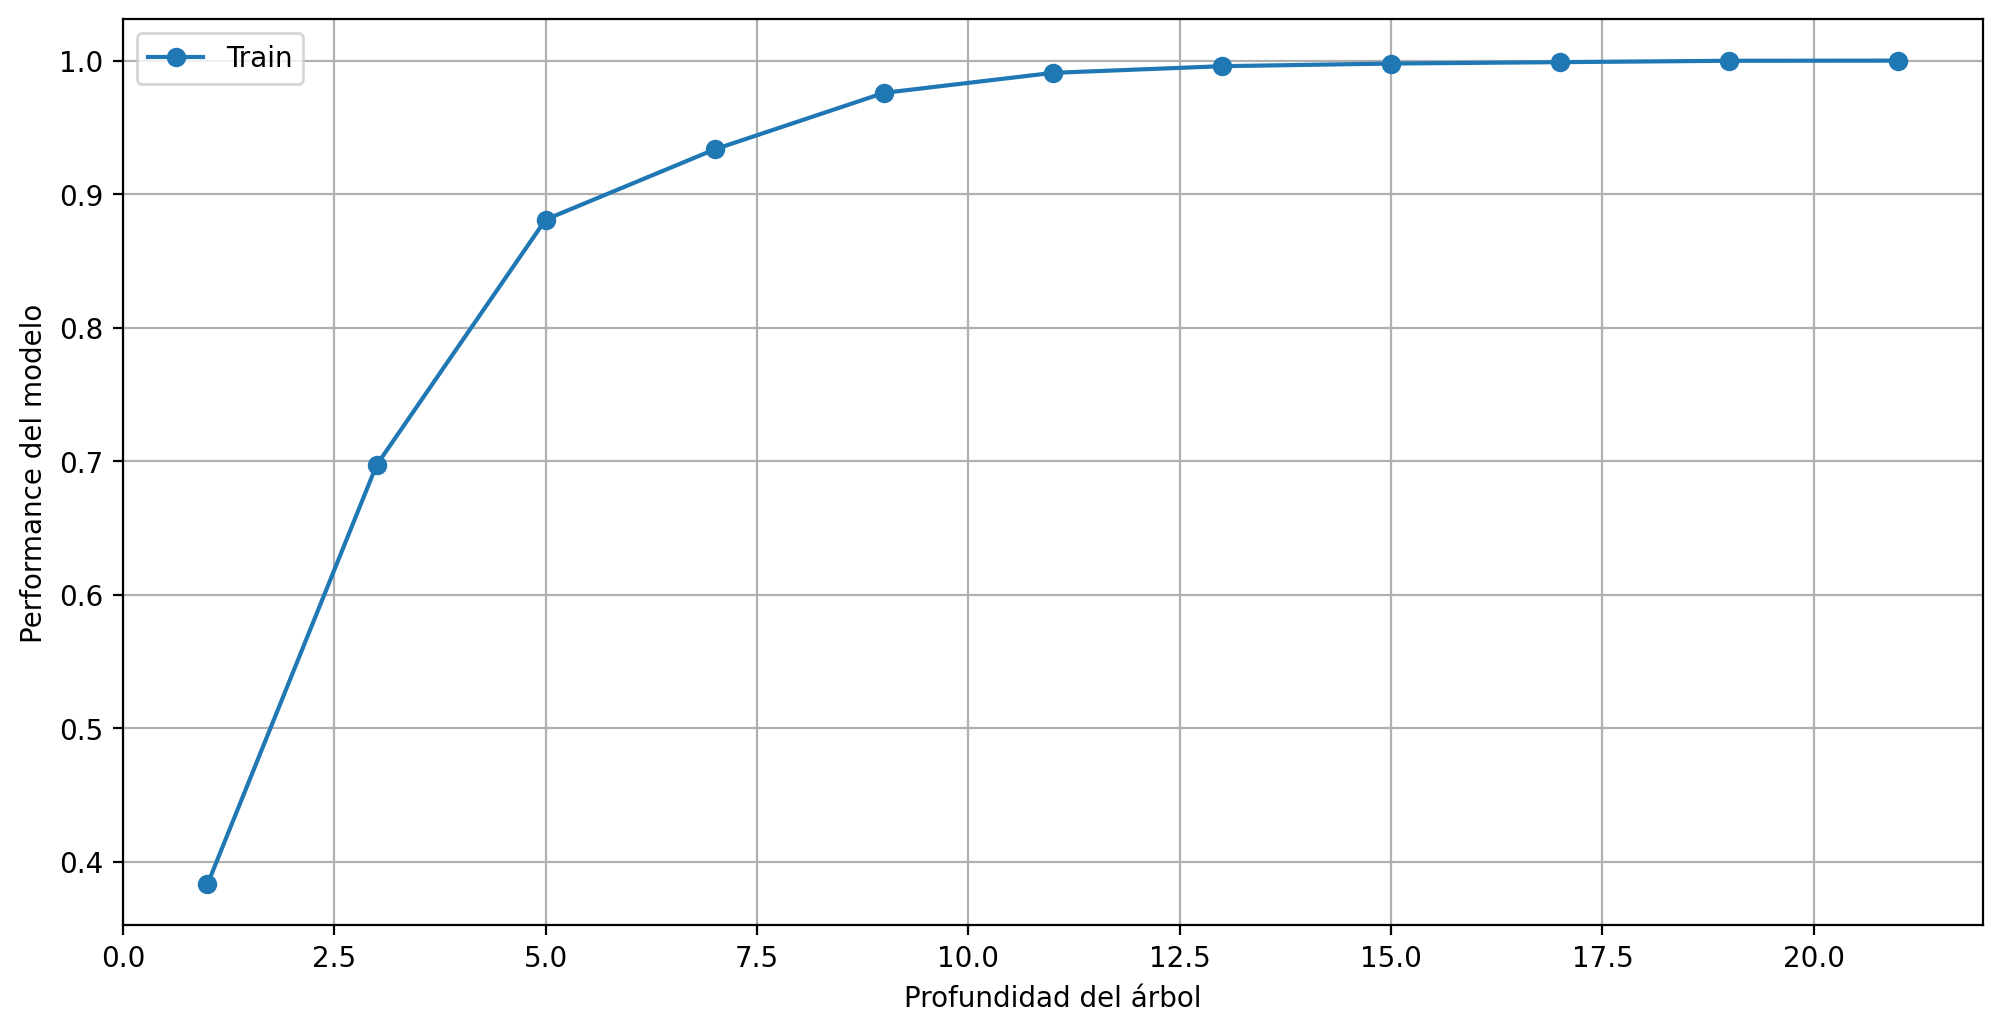
\includegraphics[scale=0.6]{figuras/3b.png}
	\caption{Performance vs profundidad del modelo de árbol de decisión}
	\label{fig:3b}
\end{figure}

Los resultados de este experimento, tal como se ve en la figura \ref{fig:3b}, mostraron que la precisión del modelo aumenta con la profundidad del árbol, lo cual es esperado. Sin embargo, es importante notar que profundidades mayores pueden llevar a sobreajuste (overfitting), donde el modelo aprende demasiado bien los datos de entrenamiento y pierde capacidad de generalización. 

	\item[]
		\textbf{Experimento 2: Validación Cruzada con K-Fold }
 
Con este experimento se busca encontrar la mejor configuración de hiperparámetros para el modelo. 

A partir del experimento anterior se pudo intuir que para encontrar la profundidad más adecuada, se podían descartar los valores muy bajos (1-6) para evitar el subajuste, y los demasiados altos (mayores a 14) para el sobreajuste. Por esto se optó por variar el hiperparámetro max\_depth entre profundidades intermedias. 
Al mismo tiempo, se buscó variar el hiperparámetro criterion para obtener la combinación óptima entre profundidad y criterio. 

Se utilizó validación cruzada con KFold (n\_splits=10, shuffle=True, random\_state=1) para evaluar el rendimiento de los modelos DecisionTreeClassifier con diferentes profundidades máximas del árbol (7 a 14) y criterios de elección de atributos (gini y entropy). 

\begin{figure}[H]
	\centering
	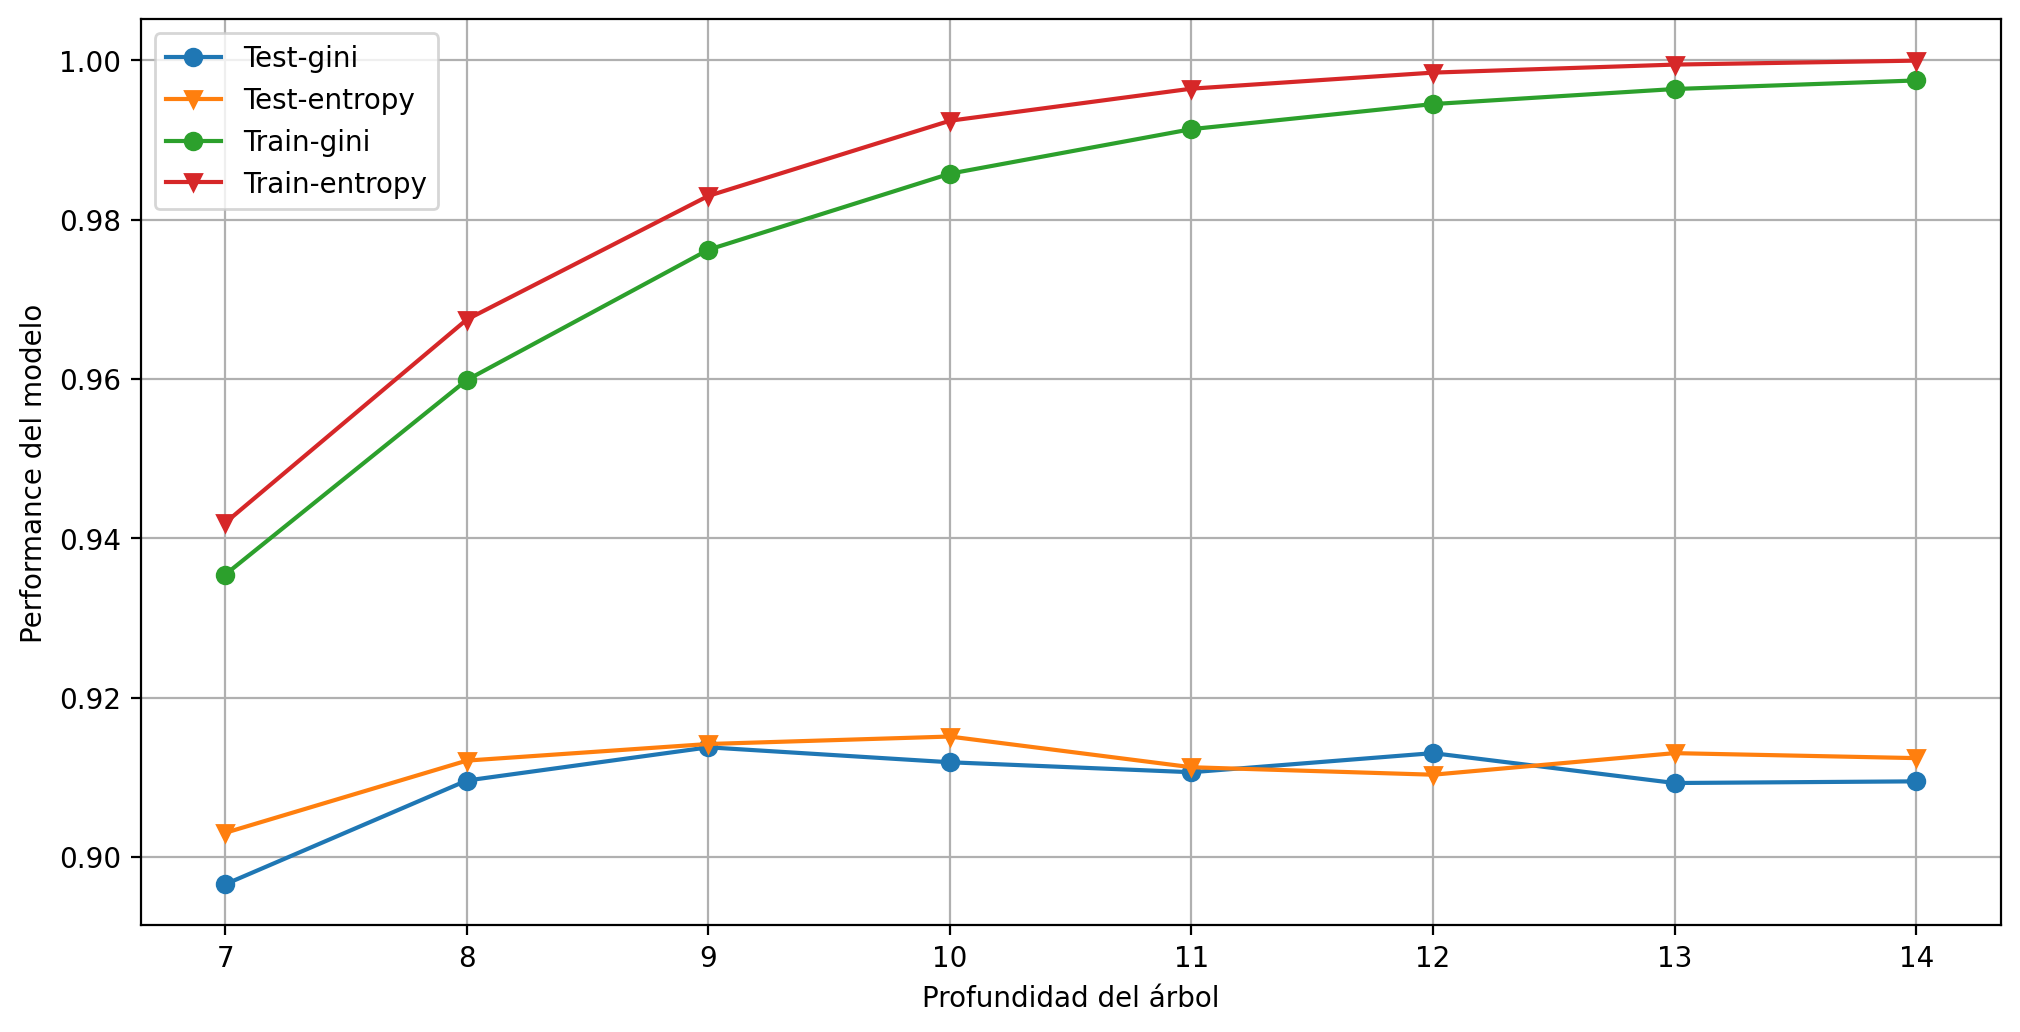
\includegraphics[scale=0.6]{figuras/3c_entropy10.png}
	\caption{Performance vs profundidad del modelo de árbol de decisión}
	\label{fig:3c}
\end{figure}

%Como se puede observar en la figura \ref{fig:3c}, 


\end{itemize}



\section{Conclusiones}



\end{document}
